\documentclass{beamer}

\usepackage[utf8]{inputenc}
\usepackage{graphicx}
\usepackage{units}
\usepackage{mathtools}

%\usetheme{Copenhagen}
\usetheme{Antibes}

% Footer with page number
\setbeamertemplate{footline}%{miniframes theme}
{
	\begin{beamercolorbox}[colsep=1.5pt]{upper separation line foot}
	\end{beamercolorbox}

	\begin{beamercolorbox}[ht=2.5ex,dp=1.125ex,
		leftskip=.3cm,rightskip=.3cm plus1fil]{author in head/foot}
		\leavevmode{\usebeamerfont{author in head/foot}\insertshortauthor}
		\hfill
		\insertframenumber
	\end{beamercolorbox}

	\begin{beamercolorbox}[colsep=1.5pt]{lower separation line foot}
	\end{beamercolorbox}
}

% Other stuff
\hypersetup{pdfstartview={Fit}}
\setbeamertemplate{caption}[numbered]

\title{3D audio source simulation on iOS devices}
\author[Orizio, Rizzini, Zucchelli]{Orizio Riccardo,\\Rizzini Mattia,\\Zucchelli Maurizio}
\date{xx july 2014}
\institute[UniBS]{University of Brescia}
\logo{
\includegraphics[width=15mm]{images/logo.png}}

\begin{document}
	\begin{frame}
		\maketitle
	\end{frame}

	\section{Overview}
	
	\begin{frame}
		\frametitle{\insertsection}
		The project goal is to realize a 3D audio simulator for the iPad.
		\begin{itemize}
			\item The interface allows to move the audio source around
			\item The interface also allows to change the orientation of the user (manipulating yaw
				and pitch of the head)
		\end{itemize}
	\end{frame}

	\begin{frame}
		\frametitle{\insertsection}
		The app is written in multiple languages:
		\begin{itemize}
			\item {\bf Ruby}, {\bf Matlab} A {\em Ruby} and a {\em Matlab} scripts are used to 
				preprocess the Database
			\item {\bf Pure Data} The audio I/O is managed using a {\em Pure Data} patch
			\item {\bf C++} The functional core of the patch is a PD external written entirely
				by us
			\item {\bf Swift} The new Apple's language for iOS devices is used to develop the
				graphical inferface of the app, which communicates with the PD patch
		\end{itemize}
	\end{frame}

	\AtBeginSection[]
	{
		\begin{frame}
			\frametitle{Outline}
			\tableofcontents[currentsection]
		\end{frame}
	}

	\section{Database Preprocessing}

	\begin{frame}
		\frametitle{\insertsection}
		\begin{itemize}
			\item The KEMAR database is a list of HRTF recorded using a manikin with two
				microphones in place of the ears
			\item Each HRTF is a couple of 128-samples FIR filters (one per ear), associated to the position
				of the source at the moment of recording
		\end{itemize}
	\end{frame}

	\begin{frame}
		\frametitle{\insertsection}
		\begin{itemize}
			\item The database is a textual file containing the data
			\item The database is processed offline and translated in three vectors containing the
				points' position, their HRTF and the result of the {\em Delaunay Triangulation}
		\end{itemize}
	\end{frame}

	\subsection{Delaunay Triangulation}

	\begin{frame}
		\frametitle{\insertsection - \insertsubsection}
		\begin{itemize}
			\item Determines a subdivision of the points' space in triangles
			\item Each triangle has the points as vertices, such that no point is left inside a triangle
			\item This subdivision allows us to search for the three points that determine the triangle enclosing the
				source with little effort
			\item The subdivision is performed thanks to a Matlab script called by the Ruby one
		\end{itemize}
	\end{frame}

	\begin{frame}
		\frametitle{\insertsection - \insertsubsection}
		\begin{figure}
			\centering
			  
\includegraphics[width=0.6\textwidth]{images/marine.jpg}
		\end{figure}
	\end{frame}

	\section{Pure Data patch}

	\begin{frame}
		\frametitle{\insertsection}
		\begin{figure}
			\centering
			  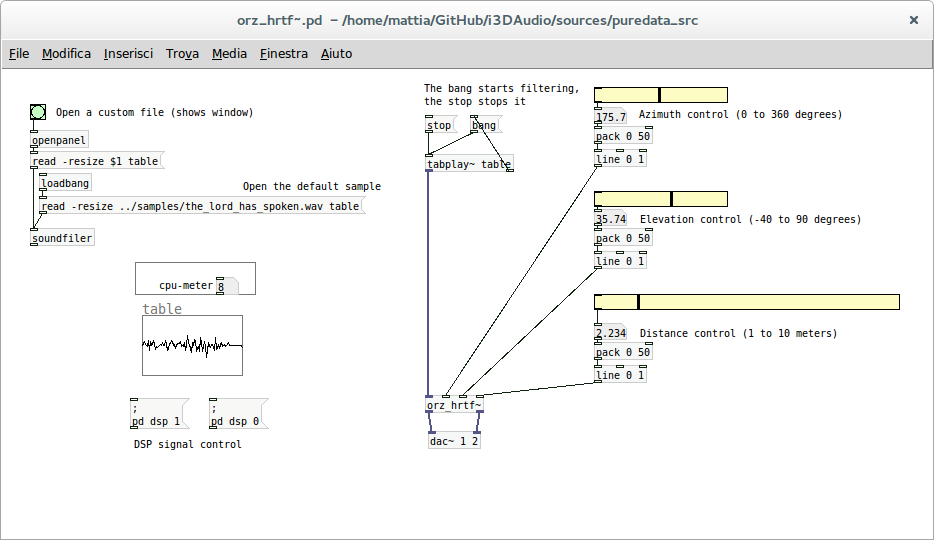
\includegraphics[width=0.7\textwidth]{images/Test_patch.png}
			  \caption{The patch used to test our external}
			  \label{fig:test}
		\end{figure}
	\end{frame}
	
	\begin{frame}
		\frametitle{\insertsection}
		\begin{itemize}
			\item The block orz$\_$hrtf$\sim$ filters the signal in the given source's position
			\item The position is given in azimuth, elevation and distance from the user
			\item The resulting outlets are the left and right channel of the filtered signal
		\end{itemize}
	\end{frame}

	\begin{frame}
		\frametitle{\insertsection}
		\begin{figure}
			\centering
			  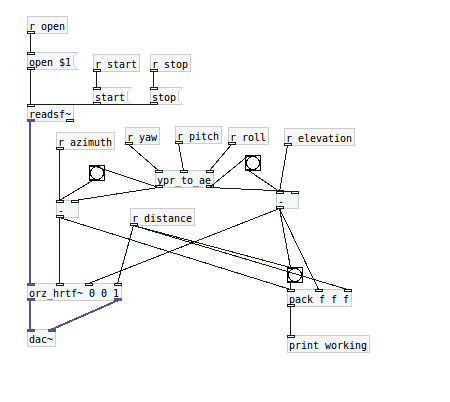
\includegraphics[width=0.5\textwidth]{images/iOS_patch.png}
			  \caption{The patch used by the app}
			  \label{fig:ios_pd}
		\end{figure}
	\end{frame}

	\begin{frame}
		\frametitle{\insertsection}
		\begin{itemize}
			\item Now the parameters are received from outside (r blocks)
			\item Also, the azimuth and elevation are modified accordingly to the given yaw and pitch of
				the head
		\end{itemize}
	\end{frame}

	\section{Processing external}

	\subsection{Structure}

	\begin{frame}
		\frametitle{\insertsection - \insertsubsection}
		\begin{itemize}
			\item A Pure Data external must be written in C (or wrapped in C++)
			\item A {\em setup} method is called when the block is loaded in the patch to initialize inlets,
				outlets and callback methods
			\item A {\em new} method instantiates the internal data of the class
			\item A callback method to handle the DSP signal must be present, in our case it is called {\em perform}
		\end{itemize}
	\end{frame}

	\begin{frame}
		\frametitle{\insertsection - \insertsubsection}
		The {\em perform} method works this way
		\begin{itemize}
			\item Find the points that form the triangle which encloses the source
			\item Determine the coefficients for the HRTF interpolation interpolate it
			\item Filter the signal separately with the left and right HRTFs
		\end{itemize}
	\end{frame}

	\subsection{HRTF interpolation}

	\begin{frame}
		\frametitle{\insertsection - \insertsubsection}
		\begin{itemize}
			\item The distance between the triangles and the source is used as a first estimate of the probability of enclosing
				the source
			\item The correct one will be the one that produces positive coefficients for the source's HRTF interpolation
		\end{itemize}
	\end{frame}

	\begin{frame}
		\frametitle{\insertsection - \insertsubsection}
		$$ HRTF_{s,l,r} = \sum\limits_{i=0}^2 g_i \cdot HRTF_{i,l,r} $$
		$$ g = H^{-1} \cdot s $$
		$$ H = [ point_0 | point_1 | point_2 ] $$
	\end{frame}
	
	\subsection{Filtering}

	\begin{frame}
		\frametitle{\insertsection - \insertsubsection}
		\begin{itemize}
			\item The filtering is a convolution of the signal with the two computed HRTFs
			\item Past filters are used to smoothen the transition from one filter to another
		\end{itemize}
	\end{frame}

	\section{The iPad interface}

	\begin{frame}
		\frametitle{\insertsection}
		\begin{figure}
			\centering
			  
\includegraphics[width=0.6\textwidth]{images/marine.jpg}
		\end{figure}
	\end{frame}

	\begin{frame}
		\frametitle{\insertsection}
	\end{frame}

	\begin{frame}
		\frametitle{\insertsection}
	\end{frame}

\end{document}
